% !TeX program = lualatex

\documentclass[]{book}
\usepackage[utf8]{inputenc}
\usepackage{natbib}
\usepackage{bibentry}
\usepackage{amsmath}
\usepackage{algorithm}
\usepackage[noend]{algpseudocode}
\usepackage{mathtools}
\usepackage{amsmath}
\usepackage{amssymb}
\usepackage{float}
\usepackage{amsthm}
\setcitestyle{square}
\usepackage{tikz}
\usepackage{booktabs}
\usepackage{enumerate}
\usepackage{yhmath}
\usepackage{chemformula}
\usepackage{graphicx,wrapfig,lipsum}
\usepackage{siunitx}
\usepackage{pgfplots}
\usepackage{epsf}
\usepackage{subcaption}
\usepackage{caption}
\usepackage{amsmath}
\usepackage{amsfonts}
 \usepackage{tabularx, booktabs, makecell, caption}
 \usepackage{siunitx}
\usepackage{hyperref}
\usepackage[all]{hypcap}
\usepackage{titlesec}
\usepackage{physics}
\usepackage{fullpage}
\newcommand{\Lagr}{\mathcal{L}}
\newcommand{\Ham}{\mathcal{H}}

\renewcommand{\figureautorefname}{\textbf{Fig.}}
\renewcommand\qedsymbol{$\blacksquare$}
\newcommand{\Hamiltonian}{\hat{H}}
\newcommand{\Wavefunction}{\Psi(\underline{r},t)}
\renewcommand{\Wavefunction}{\psi(\underline{r})}
\newcommand{\positionProj}[3]{\int_{#1}^{#2} \ket{\underline{#3}}\bra{\underline{#3}}d#3}
\newcommand{\Pstate}{\ket{\psi}}
\newcommand{\pstate}{\ket{\psi}}
\newcommand{\estate}{\ket{n}}
\newcommand{\state}{\ket{u_i}}
\newcommand{\disc}[2]{\text{D}(#1;#2)}
\newcommand{\secondx}[1]{\frac{d^2#1}{dx^2}}
\newcommand{\SE}{ \left(\frac{-\hbar^2}{2m}\nabla^2+V(r)\right)\Psi(r,t) = i\hbar\frac{\partial}{\partial t}\Psi(r,t)}
\newcommand{\TISE}{ \left(\frac{-\hbar^2}{2m}\nabla^2+V(r)\right)u_n(r) =  E_n u_n(r)}
\renewcommand{\laplacian}{\nabla^2}
\renewcommand{\grad}{\underline{\nabla}}
\renewcommand{\div}[1]{\grad\cdot\underline{#1}}
\newcommand*\circled[1]{\tikz[baseline=(char.base)]{
            \node[shape=circle,draw,inner sep=2pt] (char) {#1};}}
\renewcommand{\Re}{\mathfrak{R}}
\renewcommand{\Im}{\mathfrak{I}}
\DeclarePairedDelimiter\ceil{\lceil}{\rceil}
\DeclarePairedDelimiter\floor{\lfloor}{\rfloor}
\newtheorem{definition}{Definition}
\newtheorem*{corollary}{Corollary}
\newtheorem*{claim}{Claim}
\newtheorem*{theorem}{Theorem}
\newtheorem*{property}{Property}
\newtheorem{postulate}{Postulate}
\renewcommand{\arraystretch}{1.2}

\newcolumntype{Y}{>{\centering\arraybackslash}X}
\renewcommand{\figurename}{\textbf{Fig.}}
\makeatletter
\def\BState{\State\hskip-\ALG@thistlm}
\makeatother
\pgfplotsset{compat=1.18}
\setcounter{secnumdepth}{4}


\hypersetup{
    colorlinks=false, %set true if you want colored links
    linktoc=all,     %set to all if you want both sections and subsections linked
    linkcolor=black,  %choose some color if you want links to stand out
}


\title{Summer Project}
\author{Pablo Morandé }
\date{2023}

\begin{document}
\begin{titlepage}
    \pagestyle{empty}                       % No numbers on title page      
\begin{center}
        \vspace*{1cm}
            
        \Huge
        \textbf{Lattice Quantum Field Theory}
            
        \vspace{0.5cm}
        \LARGE
        Summer Project
            
        \vspace{1.5cm}
            
        \textbf{Pablo Morande}
        \vspace{1.5cm}


            
        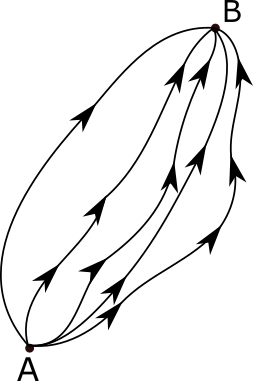
\includegraphics[width=0.4\textwidth]{Images/Feynman_paths.png}
        \vspace{1.5cm}

        \Large
        School of Physics And Astronomy\\
        The University of Edinburgh\\
        United Kingdom\\
        2023
            
    \end{center}\end{titlepage}
\tableofcontents

\pagestyle{plain} 
\setcounter{page}{1}

\chapter{Introduction}


\section{Brief Review of Classical Mechanics}
Let's consider a system described by N generalized coordinates ($\{q\}$). Given two fixed endpoints $(t_a,t_b)$ such that $\{q(t_a)\}= \{q_a\}$ and $\{q(t_b)\} = \{q_b\}$ the action of the system is defined as:
\begin{equation}
    S[\{q(t)\}] \equiv \int_{t_a}^{t_b} \Lagr(\{q\},\{\dot q\},t) dt
    \label{eq:action}
\end{equation}
Where $\Lagr$ is the Lagrangian ($\Lagr$) of the system and is defined as:
\begin{equation}
    \Lagr \equiv T(\{q\},\{\dot q\},t) - V(\{q\},t)
\end{equation}
Where $T(\{q\},\{\dot q\},t), V(\{q\},t)$ are the usual Kinetic and Potential energies respectively (expressed in terms of the generalized coordinates and possibly time). It is important to note that this definition is only useful when the system of interest is not subject to time-dependent forces. In such cases, the potential energy term must be adapted such that the right equations of motion are obtained.

\vspace{1mm}\noindent
The action, of the system is a Functional, which is a mathematical object that given a function returns a number. In this case, the action needs to be fed a trajectory $\{q(t)\}$ so that the integral in Equation \ref{eq:action} can be integrated to produce a number.

\vspace{1mm}\noindent
Once these two objects have been introduced it is time to use them to obtain a formulation of classical mechanics. The key part is to introduce Hamilton's Principle
\begin{definition} Hamilton's Principle:
This principle establishes that given  a system described by N generalized coordinates, the path that the system will take will be such that makes the action stationary and that satisfies the boundary conditions at the specified endpoints $(t_a,t_b)$. That is we require that $\delta S =0$ for the classical path.
\end{definition}
\noindent It turns out that this condition is enough to obtain a set of equations of motion that describe the mechanics of the system. To obtain these equations we need to consider the change on the action under the coordinate change $\{q(t)\} \to \{q(t) + \epsilon(t)\}$ and then we impose that this change must be zero for the classical path:
\begin{align}
    \delta S &\equiv S[\{q(t)+ \epsilon(t) \}] - S[\{q(t) \}] \\
    &= \int_{t_a}^{t_b} \Lagr(\{q+\epsilon(t)\},\{\dot q + \dot\epsilon(t)\},t) dt - \int_{t_a}^{t_b} \Lagr(\{q\},\{\dot q\},t) dt\\
    &= \int_{t_a}^{t_b} \left(\frac{\partial  \Lagr}{\partial q_i} \epsilon_i + \frac{\partial  \Lagr}{\partial \dot q_i} \dot\epsilon_i\right)dt +O(\epsilon^2) =  \int_{t_a}^{t_b} \left(\frac{\partial  \Lagr}{\partial q_i}  -\frac{d}{dt} \frac{\partial  \Lagr}{\partial \dot q_i} \right) \epsilon_i dt
\end{align}
In the last line, we have integrated by parts and we have used that the endpoints are fixed for all paths (so $\{\epsilon(t_a)\} = \{\epsilon(t_b)\} = \{0\}$. We now impose the condition for the classical path, $\delta S= 0$
\begin{align}
    \int_{t_a}^{t_b} \left(\frac{\partial  \Lagr}{\partial q_i}  -\frac{d}{dt} \frac{\partial  \Lagr}{\partial \dot q_i} \right) \epsilon_i dt = 0
\end{align}
As this condition must hold for general (but small) $\{\epsilon(t)\}$ we find that the following equations must be satisfied for the classical path:
\begin{equation}
  \frac{d}{dt} \frac{\partial  \Lagr}{\partial \dot q_i} =   \frac{\partial  \Lagr}{\partial q_i} 
\end{equation}
Which are the Euler-Lagrange Equations of Motion.

\vspace{1mm}\noindent \textbf{Example:} Free particle 


\vspace{1mm}\noindent Let's examine the case of a 1-dimensional free particle under this formalism. The Lagrangian of the system is just $\Lagr = \frac{m}{2}\dot x^2$ as there is no potential energy term and only one degree of freedom. Therefore, the Euler-Lagrange Equation is:
\begin{align}
         \frac{d}{dt} \frac{\partial  \Lagr}{\partial \dot x} &=   \frac{\partial  \Lagr}{\partial x} \\
         \ddot x &=0
\end{align}
Solving the differential equation and applying the boundary conditions $x(t_a) =x_a, x(t_b) = x_b$ gives the solution: $x(t) = \frac{x_b}{t_b-t_a}(t-t_a)+\frac{x_a}{t_b-t_a}(t_b-t) $. Which is the classical equation of motion. It is now possible to reintroduce into the Lagrangian to obtain the action of the classical path. Doing this and performing the integral gives:
\begin{equation}
    S_{\text{C}} = \frac{m}{2}\frac{(x_b-x_a)^2}{T}, T = t_b-t_a
\end{equation}
$  S_{\text{C}}$ Stands for classical action, that is the action evaluated along the classical path (for which the action is stationary).

\vspace{1mm}\noindent One of the strengths of this approach to classical mechanics compared to the Newtonian formalism is that the conservation laws are easy to obtain. At this stage, it is useful to introduce the canonical momenta. For a system described by N generalized coordinates, the canonical momenta $p_i$ with $1\leq i \leq N$ is defined as:
\begin{equation}
    p_i \equiv \frac{\partial \Lagr}{\partial \dot q_i}
\end{equation}
These quantities are important as they are the ones involved in conservation laws. If the Lagrangian of the system is independent of the coordinate $q_i$ then the conjugate momenta to that coordinate (that is $p_i$) will be conserved. This is just a trivial consequence of the Euler-Lagrange Equations:
\begin{proof}
    \begin{align}
      \frac{d}{dt} \frac{\partial  \Lagr}{\partial \dot q_i} &=   \frac{\partial  \Lagr}{\partial q_i} = 0 \\
      \frac{d}{dt} p_i &= 0 \\
      p_i &= C
\end{align}
Where C is just a constant. Therefore $p_i$ is conserved (A constant of the motion)
\end{proof}
Another important conservation law arises when the Lagrangian of the system is independent of time, that is when $\frac{\partial\Lagr}{\partial t}=0$. In this case, the energy function is conserved. This object is defined as follows:
\begin{equation}
    h(\{q\},\{\dot q\},t) \equiv \sum_{i=1}^N \frac{\partial  \Lagr}{\partial \dot q_i}\dot q_i - \Lagr(\{q\},\{\dot q\},t)
\end{equation}
Its conservation is a consequence of the chain rule and of the Euler Lagrange Equation:
\begin{proof}
\begin{align}
    \frac{d\Lagr}{dt} &= \sum_{i=1}^N\frac{\partial \Lagr}{\partial q_i}\dot q_i +  \sum_{i=1}^N\frac{\partial \Lagr}{\partial \dot q_i}\ddot q_i + \frac{\partial\Lagr}{\partial t}, \frac{\partial\Lagr}{\partial t}=0\\
     \frac{d\Lagr}{dt} &= \sum_{i=1}^N\frac{\partial \Lagr}{\partial q_i}\dot q_i +  \sum_{i=1}^N\frac{\partial \Lagr}{\partial \dot q_i}\ddot q_i\\
      \frac{d\Lagr}{dt} &= \sum_{i=1}^N\frac{d}{dt}\frac{\partial \Lagr}{\partial \dot q_i}\dot q_i +  \sum_{i=1}^N\frac{\partial \Lagr}{\partial \dot q_i}\ddot q_i \\
         \frac{d\Lagr}{dt} &= \frac{d}{dt}\sum_{i=1}^N\left(\frac{\partial \Lagr}{\partial \dot q_i}\dot q_i\right)\\
          0&=\frac{d}{dt}\left(\sum_{i=1}^N\left(\frac{\partial \Lagr}{\partial \dot q_i}\dot q_i\right) - \Lagr\right) \\
          h &=C
\end{align}
Where C is just a constant. Therefore $h$ is conserved (A constant of the motion)
\end{proof}
\noindent It is important to remark on the connection between the energy function and the energy of the system. It is not hard to show that the energy function will coincide with the energy of the system (the sum of the kinetic energy and the potential energy) if and only if the kinetic energy is quadratic on the generalized velocities. The kinetic energy of the system is said to be quadratic on their velocities if it is possible to express it as follows: 
\begin{equation}
    T = \frac{1}{2}\sum_{i,j = 1}^N \dot q_i T_{ij} \dot q_j
\end{equation}
Where $T_{ij}$ is a $N\times N$ symmetric matrix that does whose entries do not depend on the velocities.

\vspace{1mm}\noindent At this stage it is perhaps useful to introduce the Hamiltonian of the system. The Hamiltonian of a system (with N degrees of freedom), which we denote as $\Ham$, is defined as follows:
\begin{equation}
    \Ham(\{q\},\{p\},t) \equiv \sum_{i=1}^{N} p_i \dot q_i - \Lagr(\{q\},\{\dot q\},t)
\end{equation}
It is important to notice that while the definition of the Hamiltonian of the system is exactly equivalent to the definition of the energy function $h$, the Hamiltonian is defined as a function of the generalized coordinates, time and the canonical momenta and not the generalized velocities. Therefore, defining the Hamiltonian of the system is not as straightforward as it might seem as we need to transform the quantities on the right-hand side such that they are expressed in terms of the variables that define the Hamiltonian, which are the Legendre Transformations.

\vspace{1mm}\noindent \textbf{Example:} Hamiltonian of a particle in a spring. 

\vspace{1mm}\noindent Let's consider the case a 1D system of a particle in a spring, in such case the Lagrangian of the system is given by
\begin{equation}
    \Lagr = \frac{m}{2}\dot x^2 - \frac{k}{2}x^2
\end{equation}
Where $x$ is the generalized coordinate of interest (displacement from the equilibrium position) and $k$ is the spring constant. The canonical momentum conjugate to $x$, is defined as $p = \frac{\partial\Lagr}{\dot x} = m\dot x$. We now start by writing the energy function of the system:
\begin{equation}
    h = \frac{m}{2}\dot x^2 + \frac{k}{2}x^2 
\end{equation}
We know just need to change the variables that appear in $h$ to get an expression of $H$ for this system. In particular, we need to get rid of all instances of $\dot x$. In this case, we just need to replace one and we do this using the definition of the canonical momentum: $\dot x = \frac{p}{m}$. Therefore, we obtain:
\begin{equation}
      \Ham(\{q\},\{p\},t) = \frac{p^2}{2m}  + \frac{k}{2}x^2 
\end{equation}
Which is the Hamiltonian of this system.

\vspace{1mm}\noindent Now that we have defined the Hamiltonian of the system is time that we use its definition to obtain the equations of motion of the system. Let's consider a variation of the Hamiltonian $\Ham(\{q\},\{p\},t)$
\begin{equation}
    \delta H =\sum_{i=1}^N \left(\frac{\partial \Ham}{\partial q_i}\delta q_i + \frac{\partial \Ham}{\partial p_i}\delta p_i\right) + \frac{\partial \Ham}{\partial t}\delta t  
    \label{eq:HamVar1}
\end{equation}
Which is just a trivial application of Taylor's theorem. However, let's apply this definition to the right-hand side:
\begin{align}
     \delta H &= \delta\left( \sum_{i=1}^{N} p_i \dot q_i - \Lagr(\{q\},\{\dot q\},t)\right)\\
     &= \sum_{i=1}^{N} \left( p_i \delta \dot q_i + \dot q_i \delta p_i - \frac{\partial\Lagr}{\partial q_i}\delta q_i - \frac{\partial\Lagr}{\partial \dot q_i} \delta \dot q_i\right) - \frac{\partial \Lagr}{\partial t}\delta t\\
      &=\sum_{i=1}^{N} \left(  \dot q_i \delta p_i - \dot p_i \delta  q_i\right) - \frac{\partial \Lagr}{\partial t}\delta t
      \label{eq:HamVar2}
\end{align}
We now compare Equations \ref{eq:HamVar1} and \ref{eq:HamVar2} which must hold for arbitrary variations $\delta q_i,\delta p_i$ and we obtain Hamilton's Equation of Motion:
\begin{align}
    \dot q_i &= \frac{\partial \Ham}{\partial p_i}\\
    \dot p_i &= -\frac{\partial H}{\partial q_i}\\
    \frac{\partial \Lagr}{\partial t} &= -\frac{\partial H}{\partial t}
\end{align}
If we now consider a general function of the generalized coordinates and momenta such as $\mathcal{A}(\{q\},\{p\},t)$ its time evolution is given by:
\begin{equation}
    D
    \label{eq:TimeEvClassical}
\end{equation}
It is now possible to express this in terms of the Hamiltonian of the system using Hamilton's Equations described above:
\begin{equation}
    \frac{d\mathcal{A}}{dt} = \sum_{i=1}^N \left(\frac{\partial\mathcal{A}}{\partial q_i}\frac{\partial \Ham}{\partial p_i} - \frac{\partial\mathcal{A}}{\partial p_i}\frac{\partial \Ham}{\partial q_i}\right) +\frac{\partial \mathcal{A}}{\partial t}
\end{equation}
It is possible to write this in an even more compact way if we introduce the Poisson Bracket. The Poisson Bracket is an object involving two functions of the Generalized coordinates and  momenta $\mathcal{A}(\{q\},\{p\},t)$, $\mathcal{B}(\{q\},\{p\},t)$ and is defined as follows:
\begin{equation}
    \{\mathcal{A},\mathcal{B}\}_{PB} = \sum_{i=1}^N\left((\frac{\partial\mathcal{A}}{\partial q_i}\frac{\partial \mathcal{B}}{\partial p_i} - \frac{\partial\mathcal{A}}{\partial p_i}\frac{\partial \mathcal{B}}{\partial q_i}\right)
    \label{eq:PoissonBracketdef}
\end{equation}
Using the definition of the Poisson bracket the time evolution of a general function as described in Equation \ref{eq:TimeEvClassical} can be expressed as:
\begin{equation}
    \frac{d\mathcal{A}}{dt} =   \{\mathcal{A},\mathcal{\Ham}\}_{PB} +\frac{\partial \mathcal{A}}{\partial t}
\end{equation}
In particular, it is possible to express Hamilton's equations (two of them) using Poisson brackets:
\begin{align}
    \dot q_i = \{q_i,\Ham\}_{PB}\\
    \dot p_i = \{p_i,\Ham\}_{PB}
\end{align}
\section{Special Relativity Recap}
\section{Classical Fields}
\section{Introduction to Path integrals}

\chapter{Classical Field Theory}
\chapter{Quantum Field Theory}
\chapter{Markov Chain Monte Carlo for Lattice QFT}
\end{document}
